%!TEX program = xelatex
%!TEX options=--shell-escape
\documentclass[12pt]{article}

%
\usepackage[scheme=plain]{ctex}
%
\usepackage{fontspec}
%
\usepackage[margin = 1in]{geometry}

%
\usepackage[dvipsnames]{xcolor}
\usepackage[many]{tcolorbox}

%
\usepackage{amsmath}
\usepackage{amssymb}
\usepackage{amsthm}
%
\usepackage{tensor}
%
\usepackage{slashed}
\usepackage{physics}
\usepackage{simpler-wick}

%
\usepackage{mathtools}

%
\usepackage{bm}
\newcommand{\dbar}{\dif\hspace*{-0.18em}\bar{}\hspace*{0.2em}}
\DeclareMathAlphabet\mathbfcal{OMS}{cmsy}{b}{n}
%\usepackage{bbold}
\newcommand*{\dif}{\mathop{}\!\mathrm{d}}
\newcommand*{\euler}{\mathrm{e}}
\newcommand*{\imagi}{\mathrm{i}}

\renewcommand{\vec}[1]{\boldsymbol{\mathbf{#1}}}

\usepackage{caption}
\usepackage{multirow}
\usepackage{enumitem}

%
\usepackage{mathrsfs}
\usepackage{dsfont}

%
\usepackage{hyperref}
\hypersetup{
    colorlinks=true,
    linkcolor=violet,
    filecolor=blue,
    urlcolor=blue,
    citecolor=cyan,
}

%
\usepackage{graphicx}
\usepackage{subfig}
%
\graphicspath{{../figures/}}

\usepackage{listings}
\usepackage{lstautogobble}
\lstset{
    basicstyle=\ttfamily,
    columns=fullflexible,
    autogobble=true,
}

%
\usepackage{indentfirst}
%
\setlength{\parindent}{2em}
\linespread{1.25}

%
% \setmainfont{Times New Roman}

\title{Note}
\author{Feng-Yang Hsieh}
\date{}

\begin{document}
\maketitle

\section{Higgs Production}% (fold)
\label{sec:higgs_production}
    We want to apply deep learning methods to distinguish vector boson fusion (VBF) from gluon-gluon fusion (GGF) and Higgs production at the LHC.

    We want to apply the CWoLa methods, then can use the real data without knowing the true label.
% section higgs_production (end)
\section{Sample Preparation}% (fold)
\label{sec:sample_preparation}
    \subsection{Monte Carlo samples}% (fold)
    \label{sub:monte_carlo_samples}
        We consider Standard Model (SM) di-photon Higgs events produced via GGF and VBF channels at a center-of-mass energy of $\sqrt{s} = 14$ TeV. The Higgs boson events are generated using \verb|MadGraph 3.3.1|~\cite{Alwall:2014hca} for both GGF and VBF production. The Higgs decays into the di-photon final state, and the parton showering and hadronization are simulated using \verb|Pythia 8.306|~\cite{Sjostrand:2014zea}. The detector simulation is conducted by \verb|Delphes 3.4.2|~\cite{deFavereau:2013fsa}. Jet reconstruction is performed using \verb|FastJet 3.3.2|~\cite{Cacciari:2011ma} with the anti-$k_t$ algorithm~\cite{Cacciari:2008gp} and a jet radius of $R = 0.4$. These jets are required to have transverse momentum $p_{\text{T}} > 25$ GeV.

        The following \verb|MadGraph| scripts generate Monte Carlo samples for each production channel.
        \paragraph{GGF Higgs Sample Generation}
        \begin{lstlisting}
            generate p p > h QCD<=99 [QCD]
            output GGF_Higgs
            launch GGF_Higgs

            shower=Pythia8
            detector=Delphes
            analysis=OFF
            madspin=OFF
            done

            set run_card nevents 100000
            set run_card ebeam1 7000.0
            set run_card ebeam2 7000.0

            set run_card use_syst False

            set pythia8_card 25:onMode = off
            set pythia8_card 25:onIfMatch = 22 22
            done
        \end{lstlisting}
        \paragraph{VBF Higgs Sample Generation}
        \begin{lstlisting}
            define v = w+ w- z
            generate p p > h j j $$v
            output VBF_Higgs
            launch VBF_Higgs

            shower=Pythia8
            detector=Delphes
            analysis=OFF
            madspin=OFF
            done

            set run_card nevents 100000
            set run_card ebeam1 7000.0
            set run_card ebeam2 7000.0

            set run_card use_syst False

            set pythia8_card 25:onMode = off
            set pythia8_card 25:onIfMatch = 22 22
            done
        \end{lstlisting}
    % subsection monte_carlo_samples (end)
    \subsection{Event selection}% (fold)
    \label{sub:event_selection}
        The selection cuts after the \verb|Delphes| simulation:
        \begin{itemize}
            \item $n_{\gamma}$ cut: The number of photons should be at least 2.
            \item $n_{j}$ cut: The number of jets should be at least 2.
            \item $m_{\gamma\gamma}$ cut: The invariant mass of two leading photons $m_{\gamma\gamma}$ are required $\text{120 GeV} \le m_{\gamma\gamma} \le \text{130 GeV}$.
        \end{itemize}

        Table~\ref{tab:GGF_VBF_Higgs_cutflow_number} summarizes the cutflow number at different selection cuts.
        \begin{table}[htpb]
            \centering
            \caption{Number of passing events and passing rates for GGF and VBF Higgs production at different selection cuts.}
            \label{tab:GGF_VBF_Higgs_cutflow_number}
            \begin{tabular}{l|rr|rr}
                Cut                    & GGF    & pass rate & VBF    & pass rate \\ \hline
                Total                  & 100000 & 1         & 100000 & 1         \\
                $n_{\gamma}$ cut       & 48286  & 0.48      & 53087  & 0.53      \\
                $n_j$ cut              & 9302   & 0.09      & 42860  & 0.43      \\
                $m_{\gamma\gamma}$ cut & 8864   & 0.09      & 40694  & 0.41     
            \end{tabular}
        \end{table}
        
        Figure~\ref{fig:mjj_deta_distribution} shows the distributions of $m_{jj}$ (the invariant mass of the two leading jets) and $\Delta\eta_{jj}$ (the pseudorapidity difference between the two leading jets). The scatter plot of $m_{jj}$ versus $\Delta\eta_{jj}$ is presented in Figure~\ref{fig:mjj_deta_scatter}.
        \begin{figure}[htpb]
            \centering
            \subfloat[$m_{jj}$ distribution]{
                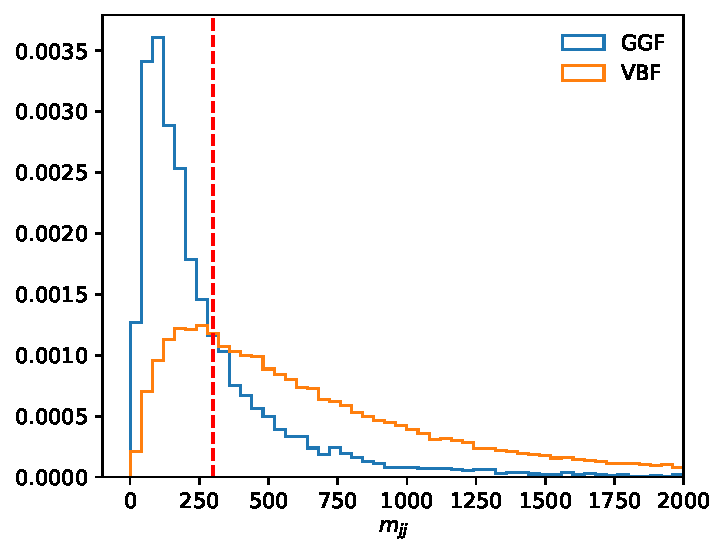
\includegraphics[width=0.45\textwidth]{mjj_distribution.pdf}
            }
            \subfloat[$\Delta\eta_{jj}$ distribution]{
                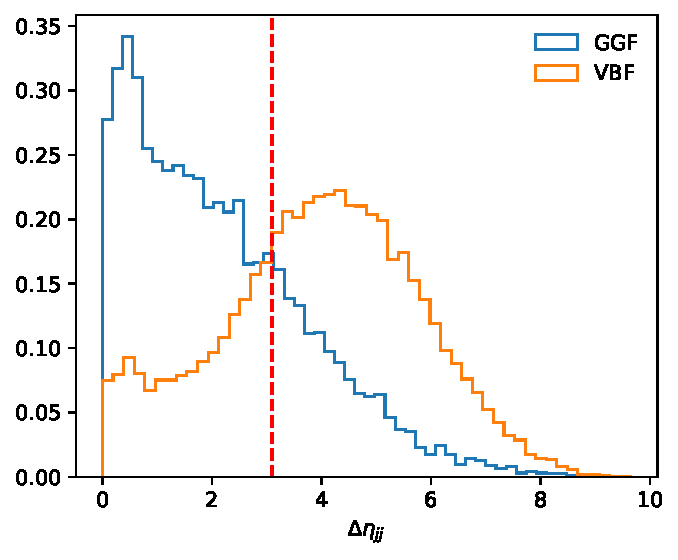
\includegraphics[width=0.45\textwidth]{deta_distribution.pdf}
            }
            \caption{Distributions of the invariant mass $m_{jj}$ and pseudorapidity difference $\Delta\eta_{jj}$ of the two leading jets. Red dashed lines are selection cuts used to construct mixed datasets.}
            \label{fig:mjj_deta_distribution}
        \end{figure}
        \begin{figure}[htpb]
            \centering
            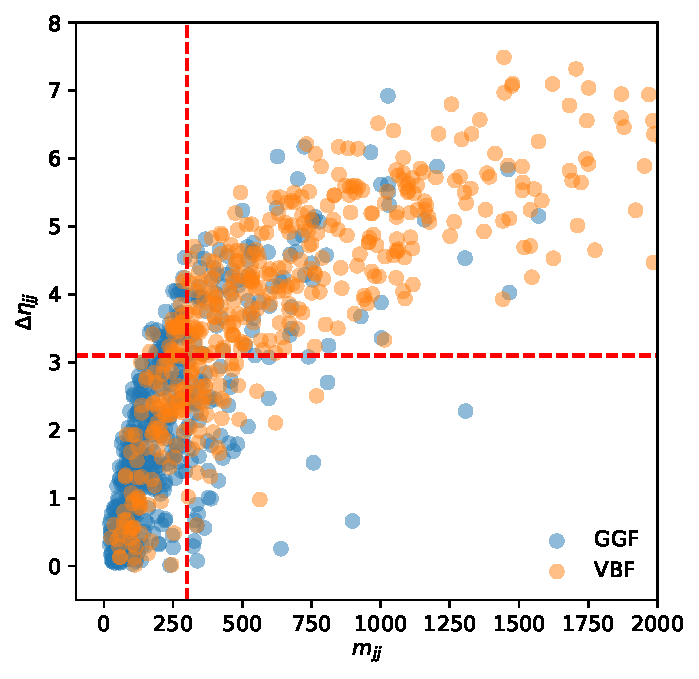
\includegraphics[width=0.45\textwidth]{mjj_deta_scatter_plot.pdf}
            \caption{Scatter plot of $m_{jj}$ versus $\Delta\eta_{jj}$. Red dashed lines are selection cuts used to construct mixed datasets.}
            \label{fig:mjj_deta_scatter}
        \end{figure}
    % subsection event_selection (end)
    \subsection{Event image}% (fold)
    \label{sub:event_image}
        The inputs for the neural networks are event images~\cite{Kasieczka:2019dbj,deOliveira:2015xxd, Kasieczka2017nv}. These images are constructed from events that pass the kinematic selection criteria described in section~\ref{sub:event_selection}. Each event image has three channels corresponding to calorimeter towers, track, and photons. The following preprocessing steps are applied to all event constituents:
        \begin{enumerate}
            \item Translation: Compute the $p_{\text{T}}$-weighted center in the $\phi$ coordinates, then shift this point to the origin.
            \item Flipping: Flip the highest $p_{\text{T}}$ quadrant to the first quadrant.
            \item Pixelation: Pixelate in a $\eta \in [-5, 5],\ \phi \in [-\pi, \pi]$ box, with $40 \times 40$ pixels 
        \end{enumerate}

        Figure~\ref{fig:GGF_VEF_event_image} shows the event images for GGF and VBF production modes.
        \begin{figure}[htpb]
            \centering
            \subfloat[GGF: Calorimeter Tower]{
                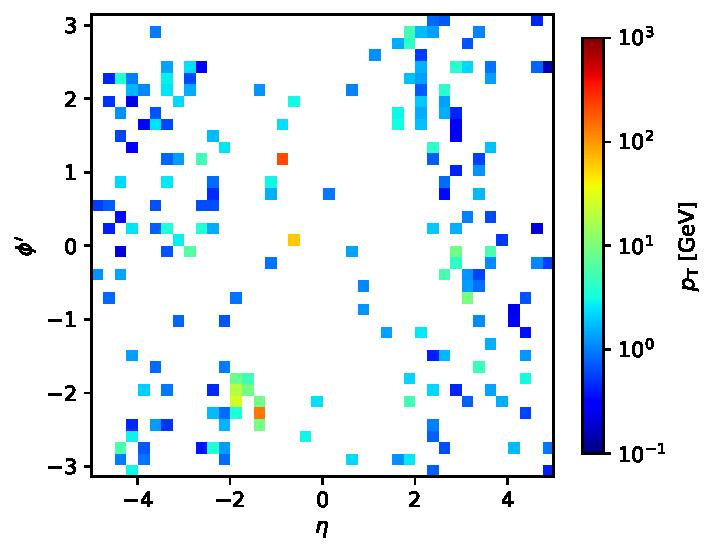
\includegraphics[width=0.45\textwidth]{event_image_GGF-tower.pdf}
            }
            \subfloat[VBF: Calorimeter Tower]{
                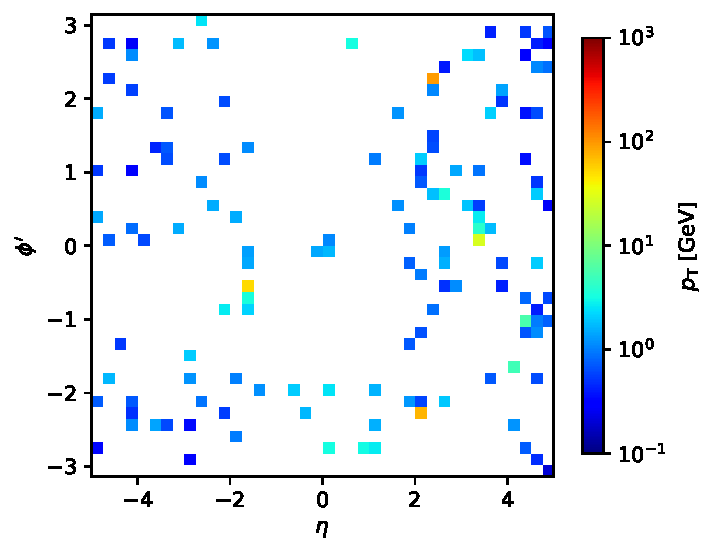
\includegraphics[width=0.45\textwidth]{event_image_VBF-tower.pdf}
            } \\
            \subfloat[GGF: Track]{
                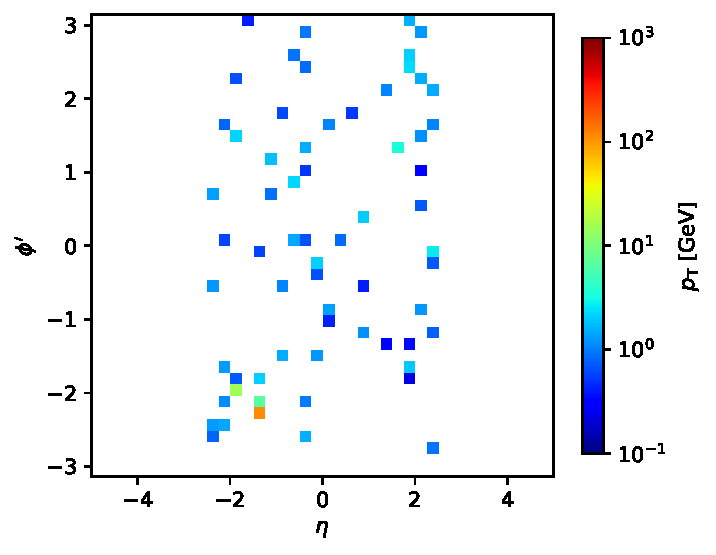
\includegraphics[width=0.45\textwidth]{event_image_GGF-track.pdf}
            }
            \subfloat[VBF: Track]{
                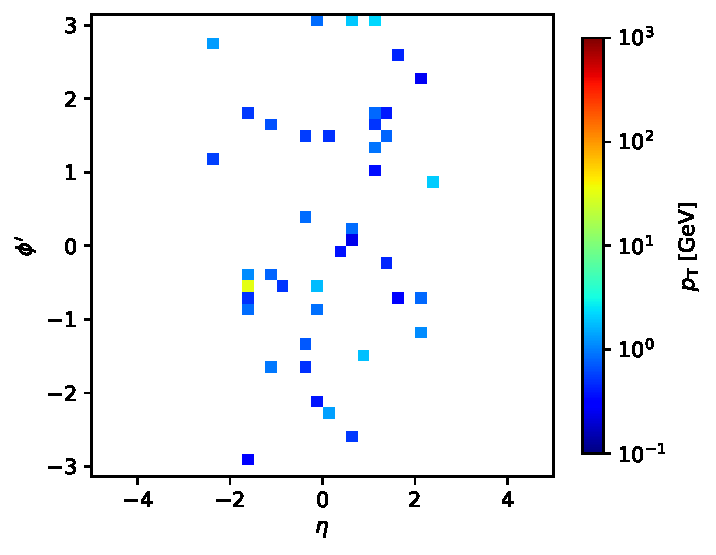
\includegraphics[width=0.45\textwidth]{event_image_VBF-track.pdf}
            } \\
            \subfloat[GGF: Photon]{
                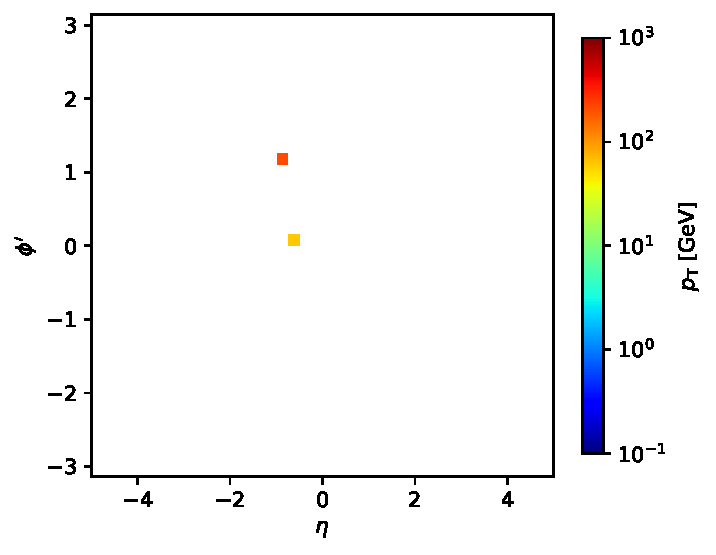
\includegraphics[width=0.45\textwidth]{event_image_GGF-photon.pdf}
            }
            \subfloat[VBF: Photon]{
                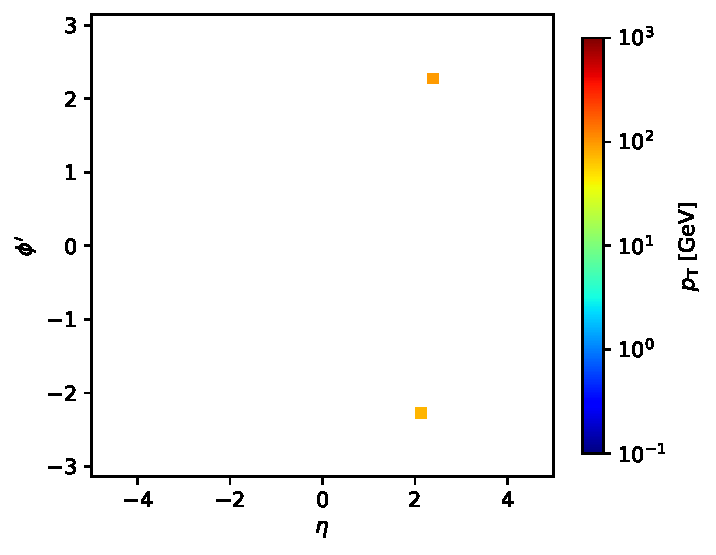
\includegraphics[width=0.45\textwidth]{event_image_VBF-photon.pdf}
            }
            \caption{Event images for GGF and VBF production, separately shown for calorimeter towers, tracks, and photons.}
            \label{fig:GGF_VEF_event_image}
        \end{figure}
    % subsection event_image (end)
% section sample_preparation (end)
\bibliographystyle{ieeetr}
\bibliography{reference}

\end{document}
